%%% Local Variables:
%%% mode: Xelatex
%%% TeX-master: t
%%% End:

\documentclass[draftformat,mathCMR]{HUSTthesis}%草稿用这个
%\documentclass[finalformat,mathCMR]{HUSTthesis}%盲审用这个

\usepackage{HUSTtils}% 所有其它可能用到的包都统一放到这里了,可以根据自己的实际添加或者删除。这样做主要是为了避免class文件过于臃肿。
% \setmainfont{Times New Roman}[Scale=.9]

\setmainfont{Times New Roman}
%\includeonly{body/chap02}

\begin{document}

%定义所有的eps文件在 figures 子目录下
\graphicspath{{figures/}}

% 生成封面,版权页,摘要

\frontmatter

%%% Local Variables:
%%% mode: Xelatex
%%% TeX-master: t
%%% End:

\ctitle{标题:宋体,英文 Times New Roman,一号,加粗,不超 30 字\\
\textcolor{red}{(中英文标题、学科专业、导师姓名正确、一致)}}

\xuehao{M2019xxxxx} \schoolcode{10487}
\csubjectname{XXXXX} \cauthorname{XXX}
\csupervisorname{XXX} \csupervisortitle{教授}
\defencedate{202X~年~X~月~X~日} \grantdate{}
\chair{}%
\firstreviewer{} \secondreviewer{} \thirdreviewer{}

\etitle{English Title,Times New Roman,小二号,实词的首字母大写\\
\textcolor{red}{中英文标题、学科专业、导师姓名正确、一致}}
\edegree{the Master Degree in Engineering} %(工学硕士)
%\edegree{the Master Degree in Science}     %(理学硕士)
%\edegree{the Professional Master Degree}   %(专业学位)
\esubject{Control Science and Engineering}
\eauthor{xxx(中文习惯,姓在前且姓全部大写)}
\esupervisor{Prof. Xxxx}

%定义中英文摘要和关键字
\cabstract{
摘要是学位论文极为重要、不可缺少的组成部分,它是论文的窗口,并频繁用于国内外资料交流、情报检索、二次文献编辑等。其性质和要求如下:
\begin{enumerate}
    \item 摘要即摘录论文要点,是论文要点不加注释和评论的一篇完整的陈述性短文,具有很强的自含性和独立性,能独立使用和被引用。
    \item 博士学位论文的摘要应包含全文的主要信息,并突出创造性成果。
    \item 内容范围应包含以下基本要素:
    \begin{enumerate}
        \item 目的:研究、研制、调查等的前提、目的和任务以及所涉及的主题范围。
        \item 方法:所用原理、理论、条件、对象、材料、工艺、手段、装备、程序等。
        \item 结果:实验的、研究的、调查的、观察的结果、数据,被确定的关系,得到的效果、性能等。
        \item 结论:结果的分析、研究、比较、评价、应用;提出的问题,今后的课题,建议,预测等。
        \item 其他:不属于研究、研制、调查的主要目的,但就其见识和情报价值而言也是重要的信息。
    \end{enumerate}
    \item 摘要的详简度视论文的内容、性质而定,\textcolor{red}{硕士学位论文摘要一般为500-600汉字。}
    \item 摘要及全文中均建议不出现“我们”等字样。摘要中主语(作用)常常省略,因而一般使用被动语态;应使用正确的时态,并要注意主、谓语的一致,必要的冠词不能省略。
    \item 一般不用图、表、化学结构式、计算机程序,不用非公知公用的符号、术语和非法定的计量单位。
    \item 摘要中一般不使用缩写词,若实在需要,在第一次使用前,需给出中文全称(缩写词);在使用英文缩写词之前,需给出英文全称(英文全称,缩写词),再次出现时可以采用中文或英文缩写词。
    \item \textcolor{red}{关键词应有3至8个,另起一行置于摘要下方,领域从大到小排列。关键词之间用分号隔开,最后一个关键词后面无标点。}
    \item 摘要、关键词采用中文宋体;英文Times New Roman;小四号。
    \item 应有与中文摘要和关键词相对应的英文摘要和关键词。英语摘要用词应准确,使用本学科通用的词汇。 
\end{enumerate}}

\ckeywords{关键词1;关键词2;关键词3}

\eabstract{This is abstract.

英文摘要字体为Times New Roman,小四,1.5倍行距。

英文摘要和关键词应与中文相对应。英语摘要用词应准确,使用本学科通用的词汇;摘要中主语(作用)常常省略,因而一般使用被动语态;应使用正确的时态,并要注意主、谓语的一致,必要的冠词不能省略。}

\ekeywords{Keyword1, Keyword2, Keyword3}

\makecover

%目录
\tableofcontents

% 对照表
\include{body/denotation}

\mainmatter
%%% mode: latex
%%% TeX-master: t
%%% End:

\chapter{绪论}
\label{cha:intro}

硕士学位论文应能表明作者确已在本门学科上掌握了坚实的基础理论和系统的专门知识,并对所研究课题有新的见解,有从事科学研究工作或独立担负专门技术工作的能力。硕士学位论文的字数一般不少于2.5万字,加上各类图表,从绪论到总结与展望的总页数一般不少于65页。否则,可能显得工作量不够饱满。

学位论文题名是以最恰当、最简明的词语反映论文中最重要的特定内容的逻辑组合。题名既要准确地描述内容,又要尽可能地精练,一般不宜超过30个字。题名一般避免使用不常见的缩略词、字符、代号和公式等。若实属必要,需要摘要中给出中英文全称与缩写。学位论文内容应结构合理、立论正确、推理严谨、文字简练、层次分明、逻辑严密、数据真实可靠。

学位论文文字排版的字号、行距、字距的大小,以版面清晰、容易辨识和阅读为原则。为统一起见,具体要求如下:
\begin{enumerate}
    \item[(1)] 论文页眉,楷体,小二
    \item[(2)] 章和节的题名用黑体,字号分别用三号和四号
    \item[(3)] 正文内容用宋体,英文用Times New Roman,小四号;行间距1.5倍;正文注意两侧对齐
\end{enumerate}

绪论部分是整篇论文的导引,应包括选题背景、意义;国内外研究概况;前人研究中存在的问题或知识空白;进而引出本文的研究设想,简要给出全文各章节的主要内容、以及章节之间相互联系。

在写作中无论是研究背景及意义,还是国内外研究现状,要做到有依据都必须引用参考文献。通常情况下,绪论部分的参考文献应占全文参考文献的百分之80以上。参考文献的顺序必须是按照在文章中出现的先后顺序进行排列。

以下简要说明一下绪论部分的内容及各级标题格式等。


\section{研究背景与意义}
\label{sec:general intro}
主要介绍与本文相关的基础知识,包括基本概念、理论、原理、方法与技术等,指出相关领域研究工作的意义。

在写作上要深入浅出,图文并茂,以便大同行也能读懂。

\subsection{**概念}

\subsection{**技术}
...

\section{XXX国内外研究现状(请拟定具体的题目)}
\label{sec:requirement}
此处应就与本文相关的国内外研究概况进行全面综述,这样相关内容在后面章节中就可以点到为止,无需再大段大段地分别介绍了。



\section{存在的问题}
\label{sec:compile}

综合当前国内外研究现状,总结现有研究中存在的问题,以便引出本文的研究内容。

在绪论中提出问题,论文的工作正是围绕这些问题而展开。


\section{本文主要内容}
\label{sec:checklist}

不同学生学位论文的类别各异,大致可分为工程类,理论类、算法研究类、仪器/工艺设计与研发类、综合类等。不同论文的章节结构各异,但每种类型的论文还是有其特定的格式。原则上,硕士论文的主体研究内容不得少于2章,加上绪论 、总结与展望,累计不得少于5章。

作为华中科技大学硕士学位论文模板,本文首先给出了不同类型的研究论文典型结构供大家参考,再根据学术出版的规范化要求,说明论文写作中的细则。全文共分为5章。主要内容如下:

第一章 绪论:简要介绍论文的研究背景、国内外研究现状、存在的问题,给出全文的主要研究内容。为了让读者更容易理解全文,建议用一个文档结构图给出各章节逻辑关系。

本文共分为5章内容,章节内容之间的关系图如图~\ref{Fig1-1}所示。

\begin{figure}[!htbp]
    \centering
    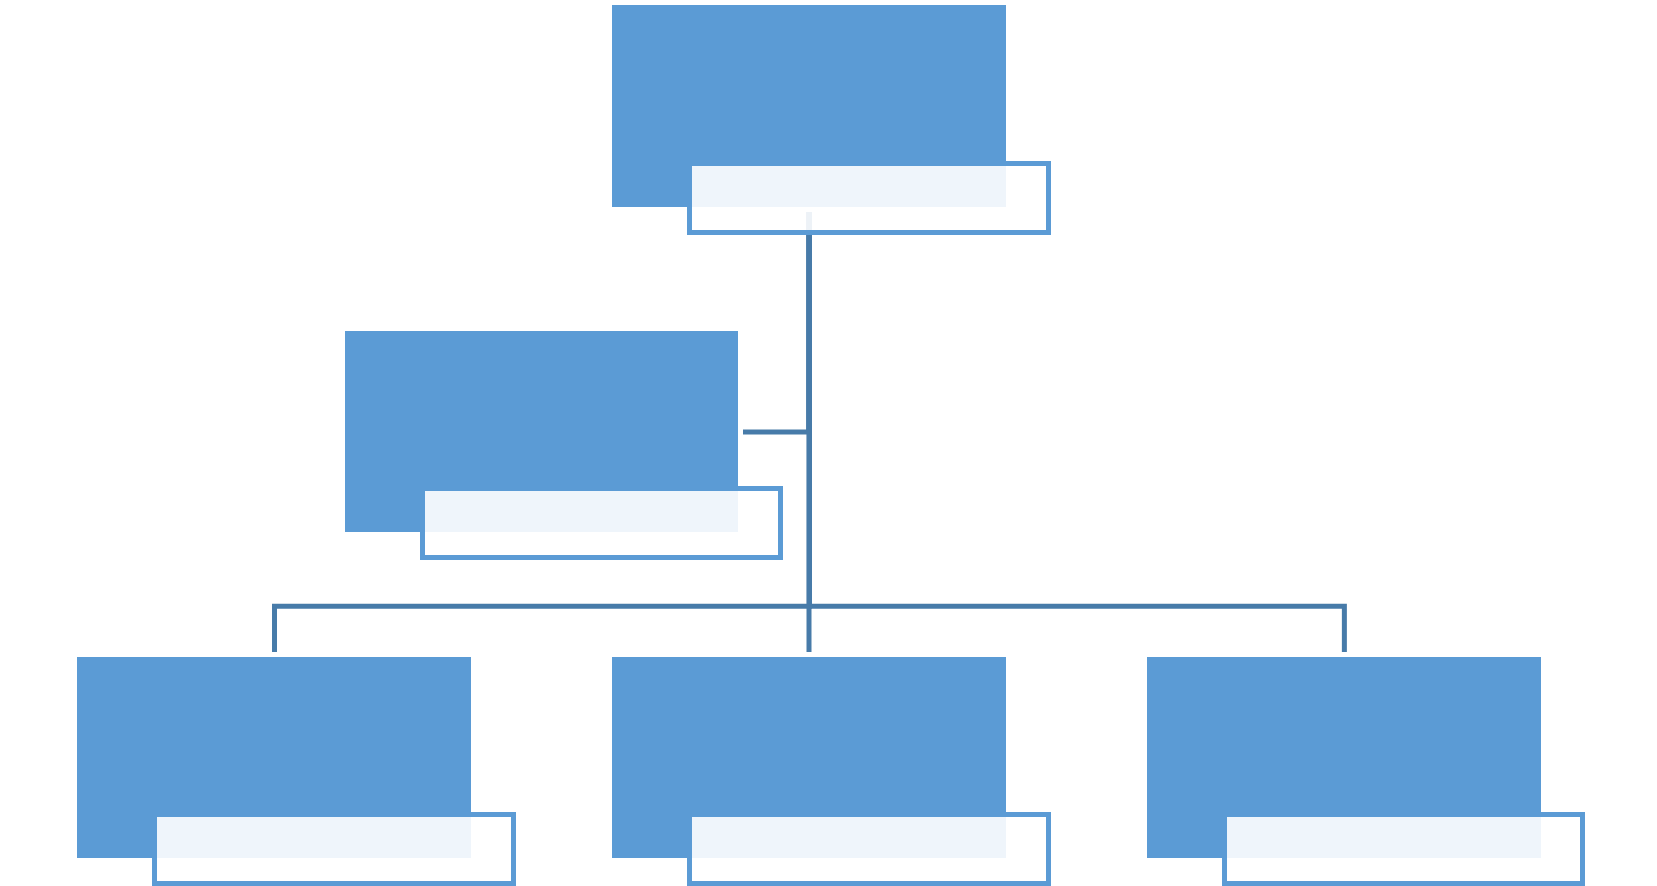
\includegraphics{figures/Fig1-1.png}
    \caption{组织结构图}\label{Fig1-1}
\end{figure}

第二章 系统与控制理论类论文结构:……

第三章 算法研究类结构:……

第四章 学位论文写作细则:……

第五章 总结与展望:给出全文的主要内容及结论,总结本文的创新点,并对未来的工作进行展望。



%%% Local Variables:
%%% mode: latex
%%% TeX-master: t
%%% End:

\chapter{系统与控制理论类论文*}
\label{cha:command}


\section{引言(引言标题可选)}
\label{sec:cover}

由于绪论中已对全文相关的研究背景和进展做了综述,因此,每章的引言中,请用1页左右的版面写一个导引,简要说明本章研究的背景或动机,以起到承上启下的作用,不宜太长。

引言的最后一段,说明本章的主要内容,如拟基于什么理论或方法,针对什么问题开展研究。注意:这里不能给结论。

若少于1个页面时,建议省略标题“引言”,直接在章的标题下写上几段话即可。

本参考模板以系统与控制理论类论文为例,各院系可根据本学科特点另行约定。

若学位论文属系统与控制理论类论文,且论文所用的基本的理论与方法基本一样,但具体应用场景不同,此时可考虑在第二章用整章的篇幅来描述,这样后面的章节就无需描重复描述相同内容,以避免冗余。

若使用的研究理论与方法并非完全相同时,建议在各章中分别介绍相关理论与方法(预备知识)、问题描述、控制策略与闭环系统分析,数值例子与实验分析,最后是小结。


\section{预备知识(可选,标题可自选)}
\label{sec:font}

\subsection{预备知识1}
陈述后续所用基本理论与方法,一般应给出相关内容来源,可引用相关文献,本部分篇幅应严格控制。给出预备知识的目的是方便大同行专家阅读理解学位论文,但要注意避免常识性或教科书基本知识的陈述。譬如,学位论文中用到深度神经网络模型,只需要叙述清楚所用的深度神经网络模型,而不需要从生物神经元、感知器模型等基础知识开始陈述。

\subsection{预备知识2}
预备知识2的相关叙述……

\subsection{预备知识3}
预备知识2的相关叙述……


\section{问题的描述(请拟定具体的题目)}
清晰的叙述本章所要研究的内容,并给出相应的数学模型与其基本假设。例如,

这里我们考虑一个由N个跟随者和一个编号为0的领导者构成的多自主体网络。其中,跟随者的动力学由如下动力学描述
\begin{equation}
\sum_{i=1}^{\left[ \frac{n}{2}\right]} \binom{x_{i,i+1}^{i^2}}
{\left[\frac{i+3}{3} \right]} \frac{\sqrt{\mu(i)^{\frac{3}{2}}
(i^2-1)}} {\sqrt[3]{\rho(i)-2}+\sqrt[3]{\rho(i)-1}}
\end{equation}
其中第i个自主体的状态$x_i (t)\in R$,f$(x_i (t))$代表非线性连续可微函数,$U_i$表示节点i的控制输入。

\textcolor{red}{(论文所有公式的按章节顺序编号,并引用)}

……

作为章节的二级标题,若直接采用“问题的描述”,则在目录中看不到有效信息。为避免出现毫无辨识度的标题,建议将所得的结果或者研究的问题作为二级标题,但也不要一幅图一节,也可以考虑将问题描述与后续的控制器设计整合一起作为一节,各节篇幅长短不宜悬殊太大。

\section{控制器设计与闭环系统分析(请根据所设计的控制器特点自行拟定具体的题目)}

\subsection{控制器设计(标题可自选)}
控制器设计的详细叙述……

\subsection{闭环系统稳定性分析(标题可自选)}
稳定性分……

\section{数值仿真(请拟定具体的题目)}
本节中…

\section{本章小结}
\label{sec:theorem}

本章主要介绍系统与控制理论类论文正文章节的框架结构。在每章的最后,都需要对该章的内容进行小结,不宜太长,建议1/2-2/3页版面较好。主要小结一下本章用什么理论或方法、做了什么事、得到的重要结果或结论。

\chapter{理论/算法类研究类论文}
\label{cha:thirdsection}


\section{引言(引言标题可选)}
\label{sec:method}
无论什么类型的论文,在章节的标题下,都需要简要说明本章研究的背景或动机,以起到承上启下的作用。若少于1个页面时,建议省略标题“引言”,直接在章的标题下写上几段话即可。

对于非会议、期刊的信息来源,若为网址,请在当页中脚注中加以标注*。

理论研究类论文,一般包括原理介绍、理论推导/或算法设计思想,再通过模拟仿真给出结果。该类论文若提出的是新理论或算法,一般应与现有理论/算法比较。当然也可以通过实验加以验证,以评估其准确性。具体内容应包括以下几个部分:



\section{**理论/算法}
\label{sec:algorithm}



\section{**仿真或算法实现}


\section{理论/算法准确性的评估}


\section{分析与讨论}

\section{本章小结}

本章简要给出理论/算法类研究论文的基本框架。在每章的最后,都需要对该章的内容进行小结,不宜太长,建议1/2-2/3页版面。主要小结一下本章用什么理论或方法、做了什么事、得到的重要结果或结论。
\chapter{学位论文写作细则}
\label{cha:fourthsection}

学位论文很多的错误源于凌乱的格式。

为规范学位论文写作,本章结合工科学位论文的特点,参照学术出版规范,就图、表制作,名词、术语、单位、符号、数量等的使用规范化进行了说明。

\textcolor{red}{(论文中所有图表清晰,字体、格式一致,图标题在图下方,表标题在表上方。图表引用和图表不跨页,确有需要跨页不超过1页)}


\section{关于图}
\label{sec:parameters}
参照CY/T 170-2019《学术出版规范 插图》标准执行。

论文中的图一般居中放置,大小要合适,宽度不得超过文字边缘,图中文字一般不大于五号;图像分辨率应尽量不低于300 dpi;若为自画图,尽量采用中文标识,图中文字经缩放后,字号不得大于五号;图注也只需加注中文,宋体,五号。若引用文献中的图,应在图注最后标注引用,图注后无需加标点符号。文中所有的图都应予编号,图序号按“章”进行编号,如图\ref{Fig4-1}所示:
\begin{figure}[!htbp]
    \centering
    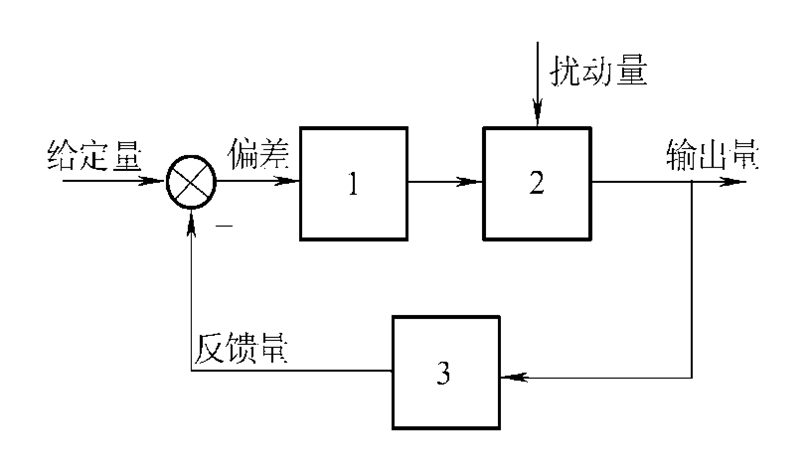
\includegraphics{figures/Fig4-1.png}
    \caption{闭环系统示意图}\label{Fig4-1}
\end{figure}
制作图时请注意:
\begin{enumerate}
    \item[(1)] 内容与形式应力求统一。风格、体例应一致。线条图应清晰,线型选用、线条粗细应规范,色调准确,图形布局合理、大小适当。连续色调图应清晰,层次感和饱和度适当。
    \item[(2)] 每幅都得有图题。图题应准确、简明地阐释该图内容。
    \item[(3)] 图应与正文内容相关。应选择能有效传达关键信息的图,应具有自明性、简明性、科学性和艺术性。
    \item[(4)] 结构示意图、原理示意图和流程图的设计制作应符合现行的国家标准或行业标准。
    \item[(5)] 坐标曲线图的坐标轴、标值线的画法应规范,标目、标值、坐标原点应标注完整、规范、统一。
    \item[(6)] 图中涉及标志用图形符号、设备用图形符号和技术文件用图形符号应符合现行的国家标准。图中的术语、数值、符号等应与正文其它图中的表述一致。
    \item[(7)] 图应尽量与相应的文字靠近,根据排版可放在文字的下方或上方。各章节不能因为图的原因出现大段留白的现象。
    \item[(8)] 图中应有对于需特别说明问题部分的标识说明,如图像中需给出比例尺,在彩图中给出Color bar等。说明字体与比例尺的字体应至少比正文小一号。
\end{enumerate}





\section{关于表格}
\label{sec:results}
学位论文中的表格要使用三线格,居中放置。表格题目应居中放置于表格顶端。仅需提供中文表头,表头及表中文字应小于正文字号,一般为宋体,五号;若其中含英文或数字时,字体为Times New Roman,五号。表格题目与表格尽量不要分页。实在需要分页时,请在下一页续表。若该表完全源于文献,应在表格题目最后标注引用。标头最后不加标点。如表\ref{Tab4-1}所示:

\begin{table}[htbp]
  \centering
  \caption{表格示例}
    \begin{tabular}{ccccc}
    \toprule
    Aaa & Bbb & Ccc & Ddd & Eee \\
    \midrule
    1-1  & 1-2  & 1-3 & 1-4 & 1-5 \\
    2-1  & 2-2  & 2-3 & 2-4 & 2-5 \\
    3-1  & 3-2  & 3-3 & 3-4 & 3-5 \\
    4-1  & 4-2  & 4-3 & 4-4 & 4-5 \\
    \bottomrule
    \end{tabular}%
  \label{Tab4-1}%
\end{table}%

一般情况下,表应放在文字的下面,有时依据排版的需要,也可以放在文字上方。但无论如何,图应尽量与文字靠近。

\begin{enumerate}
    \item[(1)] 表格序号按“章”进行编号,如第3章第1个表为“表3-1”,以此类推。
    \item[(2)] 表格内容与正文配合应相得益彰,内容适合用表表达。
    \item[(3)] 表格应具有自明性和简明性,栏目设置应科学。
    \item[(4)] 表格中的数据应具有完整性和准确性。
    \item[(5)] 表格中连续数的分组应科学,不得重叠和遗漏。
    \item[(6)] 表格中的数值修约和极原数值的书写应符合GB/T 8170的规定。
    \item[(7)] 表格中的量和单位的名称、符号及书写应符合国家标准GB3100~3102—93量和单位的系列标准和相关行业标准。
    \item[(8)] 表格中数字形式的使用应符合GB/T 15835规定。
    \item[(9)] 表格中的科学技术名词应符合CVT 119的规定。
    \item[(10)] 表格中的术语、数值、符号等应与正文以及同一文本中其他表格中的表述一致。
    \item[(11)] 全书的表格的表号、表题,表头、表身、表注的格式应统一。
\end{enumerate}

\section{名词、术语}

学位论文存在大量的专业名词与专业术语,针对同一内容的名字、术语有多种表达方式时,原则上以关系最为密切的学科为准,并尽量符合最新的国家或行业规程、规范。若属全国科学技术名词审定委员会最新公布的各类学科的“名词”,则须严格执行,且在全文中统一。

外国专有名称在释文中首次出现时,应附原文和简称。例如:“美国垦务局(United States Bureau of Reclamati,USBR)”、“美国大坝委员会(United States Committee On Large Dams,USCOLD)”。在同一条目中再次出现时可采用中文或英文缩写。


\section{符号、单位的使用}
标点符号的使用,应符合国家标准GB/T 15834—2011《标点符号用法》。
\begin{enumerate}
    \item[(1)] 论文中的计量单位应采用法定计量单位(简称法定单位),应符合国家标准GB 3100~3102—93量和单位的系列标准和相关行业标准。
    \item[(2)] 表格及插图中,使用单位符号,不使用单位名称和单位中文符号。叙述性文字中,优先使用单位符号。必要时,可使用单位名称,但不可使用单位中文符号。如:流量为11400
    \item[(3)] 两个物理量(量值加单位)在表示范围时,两个量值用波浪线“~”连接后使用一个计量单位,如:应写作800~1500 m3/s,而不写作800m3/s~1500 m3/s。
\end{enumerate}


\section{数字的使用}

数字的使用应符合国家标准GB/T15838—2011《出版物上数字用法》,同时应符合相关行业标准。

以下情况应使用阿拉伯数字:
\begin{enumerate}
    \item[(1)] 统计表中的数值,如:正负整数、小数、百分数、分数、比例。
    \item[(2)] 物理量量值,如:150 m3/s,200 kg,注意数量与单位之间应有空格。
    \item[(3)] 非物理量量值。如:21.35元,480人。
    \item[(4)] 当阿拉伯数字与汉字数字混用时,要顾及上下行文的协调一致。
    \item[(5)] 两个百分数表示范围时,要使用两个百分号,如15%~20%,不可写成15~20%。
    \item[(6)] 专业性科技出版物上的多位数字,应从小数点算起,每三位留空半个数码位置,不采用传统的以千位撇“,”分节的办法,如3800000应写成3 800 000,或写成380万,而不要写成3,800,000。
\end{enumerate}

以下情况应使用汉字数字:
\begin{enumerate}
    \item[(1)] 定型的词、词组、成语、惯用语或具有修辞色彩的词语中作为词素的数字。如:星期六、四氧化三铁、五省一市、“八五”计划、第三季度等。
    \item[(2)] 相邻两个数字并列连用表示概数,连用的两个数字间不得用顿号“、”隔开。如:二三米、十三四吨、一千七八百元。
    \item[(3)] 不是出现在具有统计意义的一组数字中的整数一至十。如:一个人、三本书、五个百分点等。
    \item[(4)] 带有“几”的数字,表示概数。如:十几天、几千年等。
\end{enumerate}

\section{其它应该注意的问题}

\subsection{关于文献引用}

在学位论文撰写中,凡是文字、图、表来自于参考文献的,必须要加注文献信息。国际惯例:与他人文章有20个字连续雷同的就是抄袭。抄袭是必须严禁的行为,否则害人害己。建议大家最好用自己的理解来撰写相关内容,特别是第一章绪论中更应注意。

在引用参考文献时,不要将文献标识直接写在某一小节的标题上,这将被视为整节内容都是引用;如有某几句话完全来自文献的,则在这部分内容的最后一句的结束加文献标注。

在课题组内部,经常出现多位同学做相近的课题,或课题的关联性较大。每个学生介绍研究背景或实验室材料与方法时,请尽可能用自己理解后的语句去撰写,以避免雷同,千万不要图省事将前一届学生的论文大段地照搬过来。有些图若是能自己画的,最好自己重新画一遍,以示区分。

\textcolor{red}{硕士学位申请人的文献阅读量一般不少于40篇,其中外文文献一般不少于1/3;近五年的论文一般不少于1/3;绪论部分应对所读文献加以分析和综合。}

参考文献格式

中文书刊:作者按中文写法,姓在前、名在后;英文书刊:作者按英文习惯写法,如名在前、姓在后,名用首字母缩写、姓用全称。一般6人以内须列出全部作者,6人以上写6人再加“等”(英文加“et al”))。每个参考文献的最后不加标点符号。

(1)图书:最多列出6个作者,作者与作者之间用逗号分隔. 书名. 版本(第×版). 译者. 出版地: 出版者, 出版年. 起页-止页(可选)

(2)期刊:最多列出6个作者,作者与作者之间用逗号分隔. 文章名. 期刊名(全称). 年号, 卷号(期号): 起页-止页或论文编号

(3)会议论文集:最多列出6个作者,作者之间用逗号分隔. 文章名. 见(英文用“in”):会议名称(或论文集). 会议城市, 国家, 会议时间, 出版者, 出版年: 起页-止页

(4)专利:专利申请者. 专利题名. 专利国别, 专利文献种类, 专利号, 出版年

(5)学位论文:作者. 题名:[博士(或硕士)学位论文]. 保存地点: 保存单位(如华中科技大学, 年份)

参考文献(举例)
\begin{enumerate}
\renewcommand{\labelenumi}{[\theenumi]}
\item	闫明礼, 张东刚. CFG桩复合地基技术及工程实践(第二版). 北京: 中国水利水电出版社, 2006

\item	M. Chalfie, S. R. Kain. Green fluorescent protein: properties, applications, and protocols. Hoboken, New Jersey: Wiley-interscience, 1998

\item	詹向红, 李德新. 中医药防治阿尔茨海默病实验研究述要. 中华中医药学刊, 2004, 22(11): 2094-2096

\item	E. S. Lein, M. J. Hawrylycz, N. Ao, M. Ayres, A. Bensinger, A. Bernard, et al. Genome-wide atlas of gene expression in the adult mouse brain. Nature, 2007, 445(7124): 168-176

\item	M. L. Bouxsein, S. K. Boyd, B. A. Christiansen, R. E. Guldberg, K. J. Jepsen, R. Müller. Guidelines for assessment of bone microstructure in rodents using micro–computed tomography. Journal of Bone and Mineral Research, 2010, 25(7): 1468-1486

\item	Y. Shunsuke, A. Masahide, K. Masayuki, M. Yoshizawa. Performance evaluation of phase-only correlation functions from the viewpoint of correlation Filters, in: 2018 Asia-Pacific Signal and Information Processing Association Annual Summit and Conference (APSIPA ASC), Honolulu, HI, USA, 12-15 Nov. 2018, Proceedings of the IEEE, 2019: 1361-1364

\item	T. Yao, J. Wan, P. Huang, X. He, F. Wu, C. Xie. Building efficient key-value stores via a lightweight compaction tree. ACM Transactions on Storage, 2017, 13(4): 1-28

\item	刘加林. 多功能一次性压舌板: 中国, ZL92214985. 2 [P]. 1993

\item	李清泉. 基于混合数据结构的三维GIS数据模型与空间分析研究[博士学位论文]. 武汉: 武汉测绘科技大学, 1998

\end{enumerate}

注释体例的基本内容、结构与位置

(1)基本内容与结构

“注释体例”含“资料性注释”和“内容性注释”两方面,合一编排。

(2)位置

正文内需注释之处依次排注号,释文于当页下部逐条依次编排。可在正文和页下注之间划一道分隔线,或通过不同的字体将二者区分开来。

(3)排版

【字体】中文:小五,宋体;英文:times new roman 9号字体;

【行距】单倍行距;

【段落】顶格写,无首行缩进,也无左缩进;

【序号】用①这种格式,序号后空一个字符,每页重新编序;

【页码】中文:第х-х页,如 第16-17页。英文:pp.х~х,如pp.5~8, 单页用pх,如p19.

【标点符号】中文使用中文状态下标点符号,英文使用英文状态下标点符号,切忌混用。

\textcolor{red}{以下是几个例子, 注意, 中文参考文献需要额外增加一个 lang="chinese"}
~\\
期刊论文举例:

Pan等人提出了一种全新的算法\cite{pan2018classification, pan2014cell, song2013asynchronous, lin2022adaptive}。

~\\
会议论文举例:

XXXXxx\cite{li2021large}

~\\
图书举例:

xxxxxx\cite{shavlik1990readings, yan2006CFG}

~\\
学位论文举例:

xxxxxx\cite{jxd1996, CCPT}




\subsection{公式}
公式中主要字母的字号与正文一样(即小四号),尽量避免图片转贴过来的公式。公式编号根据章节按顺序进行编排,如第2章第3个公式,标注为2-3,将公式编号以右对齐方式排列,但注意公式是以居中的格式排列的(类似教材中的通用格式)。

\subsection{本章小结}
本章主要介绍学位论文写作的规范化要求,包括图、表制作及其与正文的对应关系;专业名词、术语、单位、符号及数字的使用等。






%%% 结论
%%% mode: latex
%%% TeX-master: t
%%% End:

\chapter{总结与展望}
\label{cha:conclusion}

\section{本文主要内容及结论}
\label{sec:conclusion}
对全文进行全面地总结,并根据各章节归纳出若干有机联系的论点。按正文的内容分段描述,包括本研究“做了什么(提出**新理论/算法、设计或研发**工艺/仪器)、获取什么结果、得出什么结论”。

\textcolor{red}{请特别注意,全文总结与摘要及各章的小节要有所区分,不能简单的拷贝。这里的重点是结论,结论应该准确、完整、明确、精练。}


\section{本文主要创新点}
\label{sec:conclusion}
通常情况下,学位论文的创新点应放在最后一章。

创新点要凝炼,表述要清晰明了,如提出了什么创新的思路,主要特点是什么,相比现有理论或技术的提高是什么、或者有什么新的发现,是否具有重要的科学意义或应用前景。既不能过于简单,也不要太细。

硕士学位论文创新点不宜太多,一般为2个左右即可,要注意归纳创新点,千万不要以为越多越好。论文的创新不以创新点的多少来评定的,而以其创新性的价值来评定。几章的工作合在一起凝炼成一个创新点也不是不可以的。


\section{展望}
\label{sec:conclusion}
对本研究成果的意义、推广应用的现实性或可能性加以论述。同时,描述本文研究中尚存在的不足,或因时间尚未完成但又必须继续的工作,对进一步的工作进行展望。

%%% 致谢

%%% Local Variables:
%%% mode: latex
%%% TeX-master: "../main"
%%% End:

\begin{ack}

对在课题研究及论文写作过程中给予指导和帮助的导师、校内外专家、实验技术人员、同学等表示感谢。

在致谢时建议具体,不同的人如何助力完成你的论文,都需要特别注明。如导师、其他老师或实验技术人员、以及同学对你论文的贡献是不一样的,有指引课题方向、修改论文,也有具体教会实验操作,也有协助你做了哪方向的实验,或者给你精神安慰、陪你度过紧张的研究生生涯。

越具体越能表达你真实的感受,否则就是毫无意义的套话。

\end{ack}



%%% 参考文献
%Included for Gather Purpose only:
%input "ref/refs.bib"
\bibliographystyle{HUSTThesis}
\bibliography{ref/refs}



%%% 附录(根据自己实际情况增加或删减)
\begin{appendix}
%% 根据自己实际情况增加或删减
\begin{publications}
\noindent
\textbf{发表与接收论文}
\renewcommand{\labelenumi}{[\arabic{enumi}]}
\begin{enumerate}
\item Linqiang Pan, \textbf{Lianghao Li}, Ran Cheng, Cheng He, Kay Chen Tan.[J]. IEEE Transactions on Cybernetics, vol. 58, no. 6, pp. 3325-3337, 2019. (SCI源刊; IF:11.448; 署名单位: 华中科技大学)
\item \textcolor{red}{参照参考文献列出学术论文相关信息(含期刊、会议、或参编书稿),但无论有多少个作者,都必须列出全部作者名;若为英文论文,则名在前、姓在后,姓名均为全称;在本人的名字加粗,以示区别(若为第一作者,则需在最后特别注明署名华中科技大学是否为第一单位)} 
\item 若已发表,按参考文献给出页码;若只是online,给出链接;若接受或修改或投稿或拟投,也必须分别注明
\item 一般情况,一作或重要的论文放在前面
\end{enumerate}
\textbf{专\hspace{2em}利}
\renewcommand{\labelenumi}{[\arabic{enumi}]}
\begin{enumerate}
\item 全部作者的姓名全称,本人的名字加粗. 专利题名. 专利国别,专利文献种类,专利号或申请号
\end{enumerate}
\textbf{标\hspace{2em}准}
\renewcommand{\labelenumi}{[\arabic{enumi}]}
\begin{enumerate}
\item 全部作者的姓名全称,本人的名字加粗. 标准题名. 哪种层次的标准,发表年
\end{enumerate}
\textbf{科技奖励}
\renewcommand{\labelenumi}{[\arabic{enumi}]}
\begin{enumerate}
\item 全部作者的姓名全称,本人的名字加粗. 题目. 国家级/省部级科技类奖,获奖年
\item 全部作者的姓名全称,本人的名字加粗. 题目. 国际/国内竞赛类奖,获奖年
\end{enumerate}
\end{publications}
%\chapter{攻读博士学位期间参与的科研项目}
\begin{project}
\renewcommand{\labelenumi}{\textbf{\arabic{enumi}.}}
   \begin{enumerate}
    \item   \textbf{项目类型}\\  
            项目名称: 项目名称 \\
            项目编号: No. 88888888 \\
            起止时间: 2018年8月至2018年8月 \\
            担任角色:担任角色 \\
   \end{enumerate}
\end{project} 
\chapter{其他附录}

可包括详细的公式推导、实验数据、计算程序、援引他人的原始资料、数据及其设备条件等。
\end{appendix}

\end{document}
